\documentclass{article}


\usepackage{arxiv}

\usepackage[utf8]{inputenc} % allow utf-8 input
\usepackage[T1]{fontenc}    % use 8-bit T1 fonts
\usepackage{hyperref}       % hyperlinks
\usepackage{url}            % simple URL typesetting
\usepackage{booktabs}       % professional-quality tables
\usepackage{amsfonts}       % blackboard math symbols
\usepackage{nicefrac}       % compact symbols for 1/2, etc.
\usepackage{microtype}      % microtypography
\usepackage{lipsum}
\usepackage{graphicx}
\graphicspath{ {./images/} }

\author{
 Abud Santiago Elias \\
  Legajo 47015 \\
  \texttt{ sabudvicco@gmail.com} \\
   \And
 Castellano Marcelo \\
  Legajo 39028 \\
  \texttt{marce.geek22@gmail.com} \\
  \And
  Navarro Franco \\
  Legajo 46387 \\
  \texttt{franconavarro1889@gmail.com} \\
}


\title{TP 1.1 - SIMULACIÓN DE UNA RULETA}

\begin{document}
\maketitle
\begin{abstract}
Completar con un breve resumen.
\end{abstract}

% keywords can be removed
%\keywords{First keyword \and Second keyword \and More}

\section{Introducción}
La ruleta es un juego de azar típico de los casinos, cuyo nombre viene del término francés roulette, que significa ``ruedita'' o ``rueda pequeña''. Su uso como elemento de juego de azar, aún en configuraciones distintas de la actual, no está documentado hasta bien entrada la Edad Media. Es de suponer que su referencia más antigua es la llamada Rueda de la Fortuna, de la que hay noticias a lo largo de toda la historia, prácticamente en todos los campos del saber humano.

La ``magia'' del movimiento de las ruedas tuvo que impactar a todas las generaciones. La aparente quietud del centro, el aumento de velocidad conforme nos alejamos de él, la posibilidad de que se detenga en un punto al azar; todo esto tuvo que influir en el desarrollo de distintos juegos que tienen la rueda como base.

Las ruedas, y por extensión las ruletas, siempre han tenido conexión con el mundo mágico y esotérico. Así, una de ellas forma parte del tarot, más precisamente de los que se conocen como arcanos mayores.

Según los indicios, la creación de una ruleta y sus normas de juego, muy similares a las que conocemos hoy en día, se debe a Blaise Pascal, matemático francés, quien ideó una ruleta con treinta y seis números (sin el cero), en la que se halla un extremado equilibrio en la posición en que está colocado cada número. La elección de 36 números da un alcance aún más vinculado a la magia (la suma de los primeros 36 números da el número mágico por excelencia: seiscientos sesenta y seis).

Esta ruleta podía usarse como entretenimiento en círculos de amistades. Sin embargo, a nivel de empresa que pone los medios y el personal para el entretenimiento de sus clientes, no era rentable, ya que estadísticamente todo lo que se apostaba se repartía en premios (probabilidad de 1/36 de acertar el número y ganar 36 veces lo apostado).

En 1842, los hermanos Blanc modificaron la ruleta añadiéndole un nuevo número, el 0, y la introdujeron inicialmente en el Casino de Montecarlo. Ésta es la ruleta que se conoce hoy en día, con una probabilidad de acertar de 1/37 y ganar 36 veces lo apostado, consiguiendo un margen para la casa del 2.7\% (1/37).

Más adelante, en algunas ruletas (sobre todo las que se usan en países anglosajones) se añadió un nuevo número (el doble cero), con lo cual el beneficio para el casino resultó ser doble (2/38 o 5.26\%).

\section{Descripción del trabajo}
\label{sec:headings}
En este trabajo realizamos la simulación del comportamiento de una ruleta tipo Montecarlo (los números val del 0 al 36, 37 números en total) mediante un programa en Python 3.7 que carga una lista con los números que fueron saliendo en las tiradas de la ruleta, asumiendo una distribución de probabilidad uniforme discreta.

Con esos números obtenidos, procedemos luego, a calcular el promedio, el desvío, la varianza y la frecuencia relativa.

\section{Gráficas}
\begin{figure}[H]
  \centering
  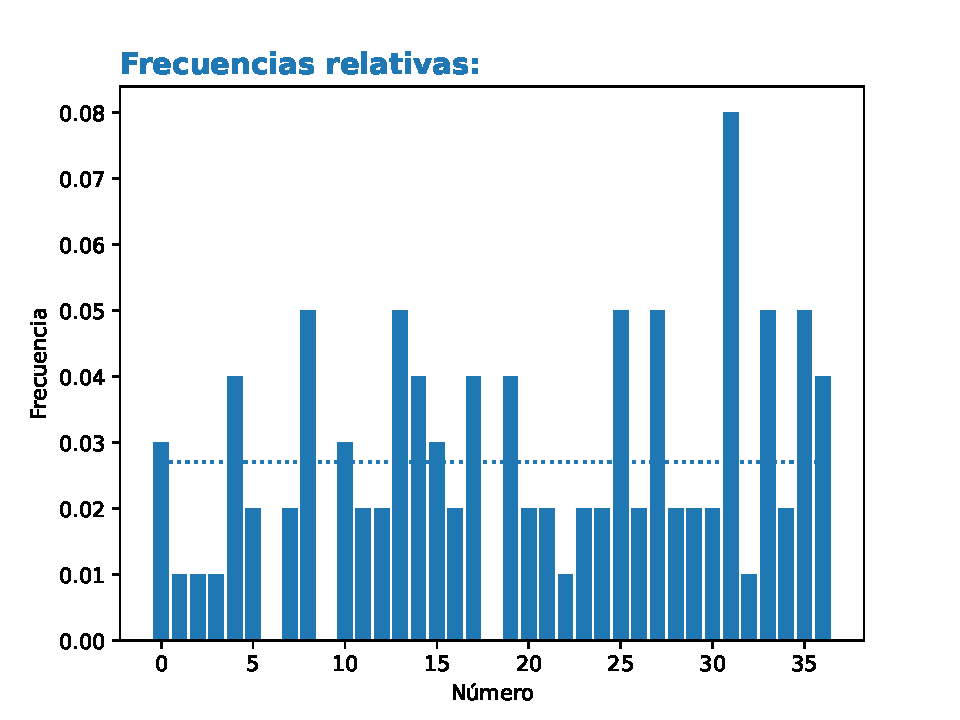
\includegraphics[width=0.3\textwidth]{frec_rel.pdf}
  %\caption{Frecuencias relativas}
  \label{fig:frec_rel}
\end{figure}

\begin{figure}[H]
  \centering
  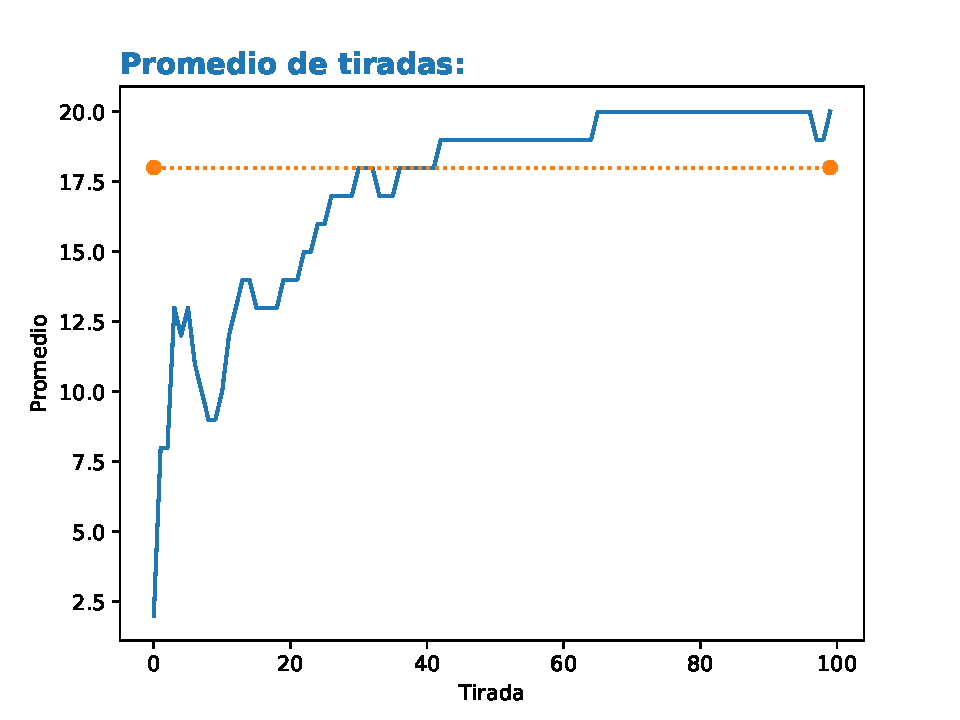
\includegraphics[width=0.3\textwidth]{promedio.pdf}
  %\caption{Promedios}
  \label{fig:promedio}
\end{figure}

\begin{figure}[H]
  \centering
  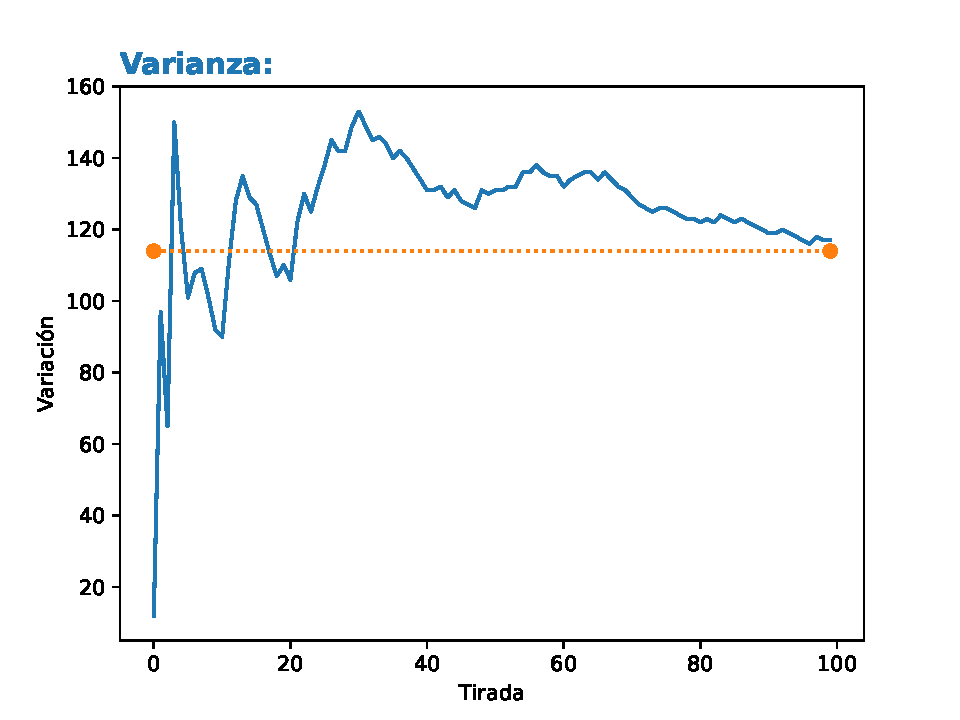
\includegraphics[width=0.3\textwidth]{varianza.pdf}
  %\caption{Varianzas}
  \label{fig:varianza}
\end{figure}

\begin{figure}[H]
  \centering
  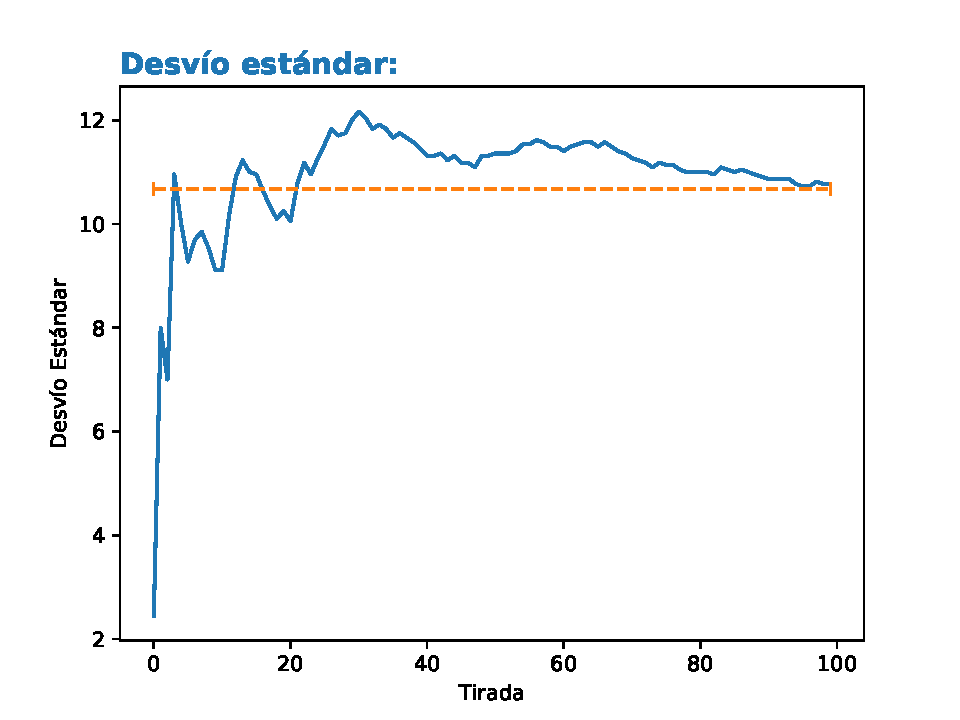
\includegraphics[width=0.3\textwidth]{desvio.pdf}
  %\caption{Desvíos}
  \label{fig:desvio}
\end{figure}

\bibliographystyle{unsrt}  
%\bibliography{references}  %%% Remove comment to use the external .bib file (using bibtex).
\end{document}
